\documentclass{report}

\usepackage{hyperref}
\usepackage[utf8]{inputenc}
\usepackage[T1]{fontenc}
\usepackage{listings}
\usepackage{graphicx}
\usepackage[brazilian]{babel}

\title{RELATÓRIO DO TRABALHO DA DISCIPLINA DE ANÁLISE DE DESEMPENHO: SIMULAÇÃO DE FILAS USANDO JMT}
\author{Mateus Regasi Gomes Martins}
\date{\today}


\begin{document}

\begin{titlepage}  
  
% faculdade no topo  
\begin{center}  
UNIVERSIDADE FEDERAL FLUMINENSE - UFF
\end{center}  
  
\vspace{8cm}  
  
% título central  
\begin{center}  
{  
ANÁLISE DE DESEMPENHO DE SISTEMAS  
}  
\end{center}  
  
\vspace{1cm}  
  
% nome deslocado para direita  
\begin{flushright}  
Mateus Regasi  
\end{flushright}  
  
\vfill  
  
% data no fundo  
\begin{center}  
Niterói -- RJ\\  
2026  
\end{center}  
  
\end{titlepage}

\section{INTRODUÇÃO}
O seguinte trabalho visa modelar e simular filas utilizando o módulo \textit{JSIMgraph} da ferramenta \textit{Open-Source} \textit{Java Modeling Tools (JMT)}, que é utilizada para esse mesmo fim. Durante o trabalho serão analisadas 4 filas básicas e será feito a comparação de suas medidas de desempenho de modelos analíticos com os simulados. Esse desenvolvimento do trabalho se dará em quatro passos:

\begin{enumerate}
    \item Fazer o download da ferramenta.
    \item Entender o funcionamento do \textit{JSIMgraph}
    \item Criar quatro modelos de fila e simulá-los através da ferramenta.
    \item Fazer um relatório dos resultados encontrados.
\end{enumerate}

Serão avaliadas métricas simples e com solução analítica. Dentre elas estão: número médio de clientes no sistema ($L$), tempo médio que um cliente passa no sistema ($W$), número médio de clientes esperando na fila ($L_Q$) e tempo médio que um cliente passa esperando na fila ($W_Q$). Outras métricas serão analisadas apenas na simulação, como fração de descarte.

A comparação será feita entre modelo simulado e analítico para avaliar a corretude do modelo simulacional. Isso ocorre pois os resultados analíticos possuem prova matemática consistente, o que os permitem serem usados para essa validação. A ideia é que se o modelo simulado gera métricas parecidas com as que esperamos pelo modelo analítico, ele provavelmente está correto.

\section{DOWNLOAD DA FERRAMENTA}

Para fazer download da ferramenta utilizada basta entrar no site oficial e clicar em \textit{Download JMT}\footnote{Acesso em: \url{https://jmt.sourceforge.net/Download.html}}. Isso iniciará o download de um arquivo \texttt{.jar}. Para instalar um programa em linguagem Java a partir de um \texttt{.jar} você necessita antes ter o \textit{Java Runtime Enviroment (JRE)} instalado em seu computador. Para isso, também é necessário instalar o JRE a partir do site oficial\footnote{Acesso em: \url{https://www.java.com/pt-br/download/manual.jsp}}. Após ter instalado o Java, estando no \textit{Linux}, basta executar o seguinte comando na pasta em que estiver o JMT: \texttt{java -jar arquivo\_baixado.jar }

Isso iniciará a instalação da ferramenta. Após instalada, basta clicar no icone que aparecerá no menu, qual conterá uma imagem escrito JMT.

\section{FUNCIONAMENTO DO JSIMGRAPH}
Como o próprio nome diz, essa ferramenta funciona como um grafo. O sistema é composto de vários elementos, que a ferramenta chama de \textit{Station}, representando os nós ou vértices do grafo. Estes são conectados através de arestas, que servem para integrar os elementos do sistema. O nó inicial é o \textit{Source}, que define o início do fluxo. A partir dele a \textit{Station} mais fundamental talvez seja é a \textit{Queue}, que é o principal elemento sobre o qual vamos trabalhar. Na \textit{Queue} você pode definir todos os parâmetros convencionais de uma fila segundo a \textit{Notação de Kendall} exceto taxa de chegada. Isto é, podemos definir: taxa ($\mu$) ou tempo de atendimento ($E[x] = \frac{1}{\mu}$), número de servidores ($C$), tamanho da fila ($K$) e política de atendimento ($P$). Outro elemento importante é o \textit{Sink}, que serve de etapa final para o nosso fluxo. O a taxa do fluxo de entrada ($\lambda$) pode ser definida por meio de uma \textit{Classe}. Com isso temos todos os elementos necessários para modelar uma fila!

Agora resta saber como se manipula as métricas. No programa elas são chamadas de \textit{performance indices}. Basta clicar no gráfico apresentado no cabeçalho do programa e definir as métricar necessárias. Para iniciar a simulação é necessário clicar no triângulo verde presente também no cabeçalho do programa.

\section{Notação de Kendall}

Seja a fila $F : A/X/C/K-P$. Segundo a notação de Kendall:
\begin{itemize}
    \item $A$ é a distribuição do tempo de chegada na fila. Pode ser: $M$ (Distribuição de Poisson), $Er$ (Distribuição Erlang) e $D$ (Determinístico);
    \item $X$ é a distribuição do tempo de atendimento da fila. Pode ser: $M$ (Distribuição de Exponencial), $C$ (Constante) e $G$ (Geral, sem distribuição específica);
    \item $C$ é o número de servidores ativos.
    \item $K$ é o tamanho da fila, pode ser um valor ou pode ser infinita. Caso seja omitida por padrão é a infinita.
    \item $P$ é a política de atendimento. Caso seja omitida, por padrão é a \textit{First In First Out (FIFO)} ou \textit{First Come First Served (FCFS)}.
\end{itemize}

\section{FORMULAÇÃO}

Em uma fila $M/M/1$:
\begin{itemize}
    \item $L_Q = \frac{\lambda ^2}{\mu(\mu-\lambda)}$ \label{eq4}
    \item $W_Q = \frac{L_Q}{\lambda}$ \label{eq5}
\end{itemize}

Pelo \textit{Resultado de Little} temos que: 
\begin{itemize}
    \item $L = \lambda W$ \label{eq1}
    \item $L_Q = \lambda W_Q$ \label{eq2}
    \item  $W = \frac{X}{1 - \lambda X}$ \label{eq3}
\end{itemize}


Em uma fila $M/M/1/K$:
\begin{itemize}
    \item Caso a fila esteja cheia (drop tail): $\lambda ' = \lambda$
    \item Caso a fila não-esteja cheia: $\lambda ' = \lambda(1-\pi_k)$
    \item $\rho = \frac{\lambda}{\mu}$
    \item $L = \frac{\lambda(1+k\rho^{k+1}-(k+1)\rho^k)}{(\mu-\lambda)(1-\rho^{k+1})}$
    \item $W = \frac{L}{\lambda'}$
\end{itemize}


\section{MODELO 1}

O primeiro modelo consiste em uma fila $M/M/1$ com $X = 1/4$ com $\frac{1}{\lambda} = \frac{1}{2}$. Foi pedido que fosse determinado $L$, $W$ e $W_Q$. Seguindo as fórmulas do modelo analítico temos que:

\begin{itemize}
    \item $W =  \frac{X}{1 + \lambda X} = \frac{1/4}{1 - 2.1/4} = 1/2$
    \item $W_Q = \frac{L_Q}{\lambda} = \frac{\frac{\lambda ^2}{\mu(\mu-\lambda)}}{\lambda} = \frac{\lambda}{\mu(\mu-\lambda)} = \frac{2}{4(4-2)}= 1/4$
    \item $L = \lambda W = 2.1/2 = 1$
\end{itemize}


\begin{figure}[h]    
	\centering
    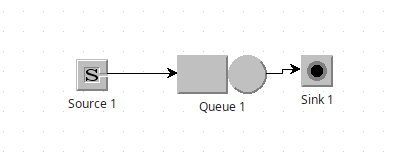
\includegraphics[width=8cm]{assets/modelo1.png}
	\caption{Primeiro Modelo}
	\label{fig:modelo1}
\end{figure}

O modelo de simulação gerou os seguintes resultados:

\begin{table}[h]
    \centering
    \caption{Resultados da fila M/M/1}
    \label{tab:modelo1}

    \begin{tabular}{|c|c|c|c|}
        \hline
        & Numbers os Customers ($N$) & Queue Time ($W_Q$) & Response Time ($W$) \\ \hline
        Max& 1.0275 &0.2522 & 0.5106 \\ \hline
        Min& 0.9756 &0.2422 & 0.4892 \\ \hline
        Avg& 1.0016 &0.2472 & 0.4999 \\ \hline
    \end{tabular}

\end{table}

Nota-se, portanto, que o resultado simulado se aproximou do resultado analítico. Mais especificamente, com um intervalo de confiança de 99\% e máximo erro relativo de 3\%.

\section{MODELO 2}

Seja um modelo $M/M/1/10$ com $X = \frac{7}{20}$ e $\frac{1}{\lambda} = 1/2$ com $drop tail$ (o cliente que chega e encontra a fila cheia vai embora). Será definido analíticamente $L$ e $W$. Pela simulação, obteremos os valores para $L$, $W$, $W_Q$ e a taxa de descarte (\textit{drop rate}).

\begin{itemize}
    \item $k = 10$
    \item $\rho = \frac{\lambda}{\mu} = \frac{2}{20/7} = \frac{7}{10}$
    \item $L = \frac{\lambda(1+k\rho^{k+1}-(k+1)\rho^k)}{(\mu-\lambda)(1-\rho^{k+1})} = \frac{2(1 + 10\times (7/10)^{11}-(11)\times (7/10)^{10})}{(20/7 - 2)(1 - (7/10)^{11})} \approx  2.1114$
    \item $\lambda ' = \lambda$ pois tem \textit{droptail}
    \item $W = \frac{L}{\lambda'} \approx 2.1114/2 = 1.0557$
\end{itemize}

\begin{figure}[h]    
	\centering
    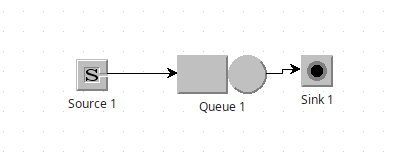
\includegraphics[width=8cm]{assets/modelo1.png}
	\caption{Segundo Modelo}
	\label{fig:modelo2}
\end{figure}

Note que a topologia do seguindo modelo é exatamente igual ao do primeiro. A única coisa que vai mudar são os parâmetros da fila. Os resultados da simulação são apresentados a seguir:

\begin{table}[h]
    \centering
    \caption{Resultados da fila M/M/1/10}
    \label{tab:modelo1}

    \begin{tabular}{|c|c|c|c|c|}
        \hline
        & Numbers os Customers ($N$) & Queue Time ($W_Q$) & Response Time ($W$)  & Drop Rate \\ \hline
        Max& 2.1416 & 0.7361 & 1.0885 & 0.0175 \\ \hline
        Min& 2.0205 & 0.6934 & 1.0400 & 0.0166 \\ \hline
        Avg& 2.0811 & 0.7147 & 1.0643 & 0.0171 \\ \hline
    \end{tabular}

\end{table}

Note que neste caso os resultados de $N$ e $W$ também bateram. Portanto o modelo de simulação está provavelmente correto.


\section{MODELO 3}

Seja a fila $M/M/5$ com $X = 1$ e $\frac{1}{\lambda} = \frac{1}{4}$. Serão considerados as métricas $L$, $W$ e $W_Q$.


\begin{itemize}
    \item Seja $W_i$ o tempo médio gasto em cada fila com $\lambda_i = 1/5 \lambda = 4/5$. Temos que $W_i =  \frac{X}{1 - \lambda_i X} = \frac{1}{1-4/5} = 5$. Como as filas estão rodando em paralelo: $W = W_i = 5$ 
    \item $L_i = \lambda_i W_i = 4/5 \times 5 = 4$. Como cada fila tem $4$ itens, então as 5 filas juntas tem 20 itens $L = 5\times L_i = 5\times 4 = 20$
    \item $W_Q = \frac{L_{iQ}}{\lambda_i} = \frac{\frac{\lambda_i ^2}{\mu(\mu-\lambda_i)}}{\lambda_i} = \frac{\lambda_i}{\mu(\mu-\lambda_i)} = \frac{4/5}{1(1-4/5)} = 4$.
\end{itemize}

\begin{figure}[h]    
	\centering
    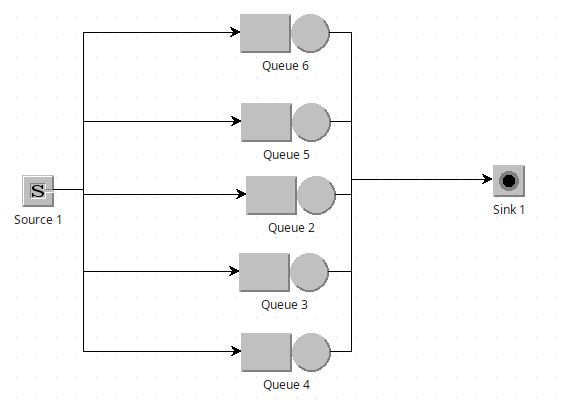
\includegraphics[width=8cm]{assets/modelo3.png}
	\caption{Terceiro Modelo}
	\label{fig:modelo3}
\end{figure}

Veja a seguir os resultados do modelo de simulação:

\begin{table}[h]
    \centering
    \caption{Resultados da fila M/M/5}
    \label{tab:modelo3}

    \begin{tabular}{|c|c|c|c|}
        \hline
        & Numbers os Customers ($N$) & Queue Time ($W_Q$) & Response Time ($W$) \\ \hline
        Max& 21.0821 & 4.0492 & 5.1306 \\ \hline
        Min& 19.2123 & 3.8272 & 4.8784 \\ \hline
        Avg& 20.1472 & 3.9382 & 5.0045 \\ \hline
    \end{tabular}

\end{table}

Note que os resultados dos modelos batem com os resultados analíticos, portanto a simulação computacional provavelmente está correta.


\section{MODELO 4}

Sejam as filas $F_1 = M/M/1$ e $F_2 = M/M/1$ em sequência com $\frac{1}{\lambda} = \frac{1}{2}$, $X_1 = \frac{1}{3}$ e $X_2 = \frac{1}{4}$. Serão definidos $L$ e $W$.

\begin{itemize}
    \item $W_1 = \frac{X_1}{1 - \lambda X_1} = \frac{1/3}{1 - 2 \times 1/3} = 1$
    \item $W_2 = \frac{X_2}{1 - \lambda X_2} = \frac{1/4}{1 - 2 \times 1/4} = 1/2$
    \item $W = W_1 + W_2 = 1 + 1/2 = 3/2$
    \item $L = \lambda W = \lambda (W_1 + W_2) = 2 \times (1 + 1/2) = 3 $
\end{itemize}

Segue a topologia do modelo:

\begin{figure}[h]    
	\centering
    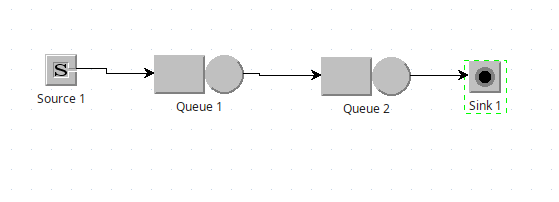
\includegraphics[width=8cm]{assets/modelo4.png}
	\caption{Quarto Modelo}
	\label{fig:modelo4}
\end{figure}

Após ter rodado as simulações, esse foi o resultado:

\begin{table}[h]
    \centering
    \caption{Resultado de 2 filas M/M/1 em série}
    \label{tab:modelo4}

    \begin{tabular}{|c|c|c|}
        \hline
        & Numbers os Customers ($N$) & Response Time ($W$) \\ \hline
        Max& 3.0681 & 1.5328 \\ \hline
        Min& 2.9241 & 1.4561 \\ \hline
        Avg& 2.9961 & 1.4944 \\ \hline
    \end{tabular}

\end{table}

Nota-se que os resultados da simulação se aproximam do modelo analítico, portanto, o modelo de simulação parece estar correto.

\section{CONCLUSÃO}

Dados os resultados, vemos que a simulação e a formulação analítica concordam entre si. Como a forma analítica tem prova matemática, os modelos simulados foram modelados corretamente.




\end{document}